\documentclass[12pt]{article}
\usepackage[a4 paper, portrait, margin=0.75in]{geometry}
\title{EGYPT\\Farmers to Pharoahs}
\author{Derrick Diana\\Harry Heathcock\\Kaedon Jon Williams}
\date{\today}
\usepackage{multicol}
\usepackage{graphicx}
\graphicspath{ {Figures/} }

\begin{document}
	\maketitle
	\begin{abstract}
			
	\end{abstract}
	
	\section{Introduction}
		Studying ancient civilisations can be difficult due to incomplete information and an inability to test hypotheses. This is a problem which can be partially solved by simulation, if the simulation can be shown to be accurate. A programme was created to reimplement an older simulation model for ancient Egyptyian farming communities in a new language to allow for extensibility and speed improvements, as well as improving the user experience. Another goal was to test whether the model was resilient to slight changes that would be resultant from a reimplementation.\\
		The simulation itself could provide assistance to researchers attempting to study ancient Egypt, allowing them to view how the conditions that were discovered came about in the first place. This could provide insight as to whether slight changes in initial conditions would create a different environment entirely.\\
		The simulation itself is an agent based model, where households claim and farm fields around the Nile River for the grain which they need to survive. Households are each part of a Settlement, which can contain many households. Households grow and thrive, while others die out.\\
		The design process used followed a few steps. The first step was to read and understand the original source code, collecting required functionality and trying to piece together how the system worked as a whole. Once the system was understood, step two began, in which the basic pieces were implemented into an object-oriented python version. This was split into the simulation and the UI, with the simulation very closely following the original code and the UI using the original as a style guide. Once the basics of the simulation and the UI had been created, a set of available data was agreed on and the two systems were brought together. The UI code instantiated a copy of the simulation code, pulled the data required for rendering each year and called the function which causes the simulation to continue for another year. From there, the final step was just to continue programming features into the simulation and UI separately until both fulfilled the original requirements.
	\section{Requirements}
		\subsection{Functional}
		\subsection{Non-Functional}
		\subsection{Usability}
		\subsection{Use Cases}
			\subsubsection{As an Archaeologist/ general user wanting to run the simulation}
				I want to be able to change input parameters before running the program to see how the results of the program are affected. Resolution: To do this, the user may select and drag any of the sliders on the left before the simulation has started running, and on doing so the simulation will reset the simulation with the changed inputs.
			\subsubsection{As an Archaeologist/ general user wishing to analyse results}
				I want to save one or more of the displayed graphs for later analysis. Resolution; To do this, the user may either save individual figures by clicking the save icon under the figure or clicking the Save All Figures button.
			\subsubsection{As an Archaeologist/ general interested experimentalist}
				I want to be able to run a large number of simulations, analyse and compare the data from different runs. Resolution: the inclusion of a Run Multiple button which allows the user to run the entire simulation as many times as the user wishes and the output graphs from each run are each saved in their own folder, within a larger containing outer folder.
			\subsubsection{As an Archaeologist/ general interested experimentalist}
				I want to be able to view details about the internal state of the system at any time in order to see how parameters change from one year to the next. Resolution: the user may pause the simulation and then right click on any block that they wish to see the parameters of. This will cause a pop-up to appear next to the block displaying information about the block. 
		
	\section{Design Overview}
		The programme was designed such that the only interactions between the simulation itself and the UI are in instantiation, the increase of years and the current state of the simulation. This was done for encapsulation purposes and to ensure the integrity of the simulation at all times. The display is split up into the UI and the rendering of the simulation, this was performed for ease of upkeep, as combining the two would result in a monolithic structure which is difficult to work with and maintain. The basic structure is shown in Figure \ref{fig:Architecture}.\\
		Due to this being a reimplementation of work that has already been done, the algorithms and data structures were pre-determined. All changes made to the overall algorithm were due to efficiency concerns, or strange behaviour which was corrected.\\
		Data was stored almost exclusively in lists, as order needed to be randomised each tick to remove possible biases due to ordering of operations being performed on the households.\\
		
		\begin{figure}[!htb]
		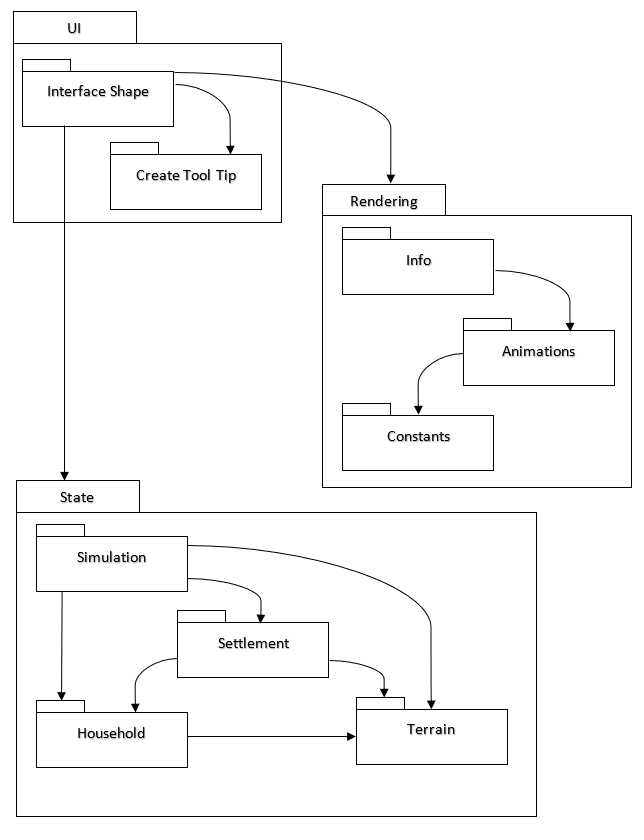
\includegraphics[width=10cm]{ArchitectureDiagram}
		\caption{Architecture diagram for the system, showing how the UI checks the state of the simulation and passes this to be rendered.}
		\label{fig:Architecture}
		\end{figure}
	
		\subsection{Changes}
			A number of changes in the implementation were made, some due to what seemed to be implementation errors in the original code and others due to functionality not making sense with what was trying to be achieved. Those which affect functionality have been implemented as explained, however when the Legacy Mode setting is enabled, these changes are reverted back to how they were in the original implementation.
				\subsubsection{Death Due to Lack of Grain}
				In the original NetLogo code, if a household did not have enough grain to survive a year then a single person would die and the grain would be set to zero. In reality this doesn't make sense, as if a household has no food, then no one would survive. The reimplementation changed this so that only the family members who can be fed will survive.\\
				\subsubsection{Population Increases}
				In the original code, if the total current population is less than or equal to the historical projected population then the population can increase. At first glance this seems to be correct, however this allows the population to always grow slightly faster than the projected historical value, and thus in the reimplementation this is changed so that the population will only increase if it is less than the historical projected population.\\
				\subsubsection{Generational Changes in Ambition and Competency}
				In the original code, if the ambition or competency for a household moved out of the bounds set (minimum, up to 1) then a new value would be generated until it fell within the bounds. This means that the computational time for the ambition and competency changes are unbounded. In the reimplementation, a value within the possible range is generated.\\
				\subsubsection{Order of Field Claimants}
				In the original code, households claimed fields in ascending order of how much grain they currently have. This seemed inconsistent with every other operation being independent of grain or ordering, in the reimplementation, this ordering is randomised each year.
	\section{Implementation}
		As can be seen in Figure \ref{fig:Packages}, InterfaceShape is the controller class which invokes other methods in all other classes. InterfaceShape contains the code which sets up the GUI, which consists of the components explained below.\\		
		A canvas object on which the main simulation grid is drawn. The main simulation grid displays the households, fields and rivers distinctly and clearly. A panel, that consists of slider and check-box objects, which allows the user to initialise parameters for the simulation. Two FigureCanvasTkAgg() objects which act as widgets and each create a matplotlib-style interactive graph. These graphs can be zoomed, scrolled, and can save their displays as images. These are live representations of figure objects within the matplotlib.pyplot library. Several other buttons and sliders which allow the user to interact with the program in minor ways.\\
		
		\subsection{Important Functions in the GUI and Rendering}
			The GUI has a method called MainLoop, which performs the primary actions corresponding to one year of the simulation which includes calling the following methods, in order:
			\begin{itemize}
				\item Simulation.tick()\\
				Which causes the simulation class to simulate a single year, generating and setting fertility values for the entire set of land, allowing households to claim, farm and rent land, as well as consuming grain, dying out when not enough food is present, allowing for population growth as well as shifts in the household competency and ambition levels.
				\item Info.drawGridSimulation()\\
				Which accesses the simulation object, finding the positions and values for fields and settlements in order to render them on the canvas correctly.
				\item Info.plotData()\\
				Which reads the necessary data out of the simulation object and appends all the data needed for each graph to a list which stores the lists required for each graph. This outer list consists of 11 inner list, each corresponding to a single graph.
				\item Info.updateGraphs()\\
				Which takes the data which has already been stored and adds it to the pyplot.figure objects which the FigureCanvasTkAgg() represent. In order to reduce the time taken to draw all the points, only points which have been added since the last draw are drawn each cycle. This is performed until the user decides to change which graph is being displayed, in which case the entire graph must be redrawn, or many lines have already been drawn, in which case the graph is redrawn as a single line. The second part is a speed optimisation, as plotting many points at once is a slow process, however the fragmentation that is created when many smaller lines have been drawn can cause the process to slow even further.
				\item Info.showGraphs()\\
				Which calls show on both of the FigureCanvasTkAgg() objects to show the data to the user.
			\end{itemize}
			
			The MainLoop method then calls itself again in a non-recursive manner using the tkinter method after(), which calls the MainLoop function again without blocking after a given delay in milliseconds. This number of milliseconds for the delay is determined by a slider that is present in the GUI and the delay is calculated each frame to achieve the desired frames per second. If the desired framerate cannot be achieved, then the programme does not sleep.
		
		\subsection{Important Functions in the Simulation}
			\subsubsection{Simulation}
				The most important function of simulation is tick(). This calls all other functions which are required for the simulation to run for a single year, incrementing all values which need to be incremented. This begins by calling flood(), which sets fertility values in the land. The settlement tick is then called, which is described below, followed by the rentLand() function. The rentLand() function sorts all the households by ambition and allows ambitious households to farm extra land which they don't own. The settlement tock function is then called, also described below.
				
			\subsubsection{Settlement}
				The two most important functions of the settlement are tick() and tock(). The first consists of functions which should be called before land rental can occur, while the latter consists of the functions which should be called afterwards. The tick() function causes each household within the settlement to claim land, and then farm their claimed land. The tock() function causes each household within the settlement to consume grain for the year, and then allows for a change in ambition and competency, as well as allowing for population growth if other values are also met.\\
				
			\subsubsection{Household}
				All of the functions in the Household class are important for the functioning of the simulation, as these are where the individual actions are controlled. The farm() function causes the household to farm its fields, the claimLand() function causes the household to make an attempt at claiming fields in the nearby area, grainTick() consuming grain for the year, populationIncrease() giving the possibility of increasing the population and generationalChange() allows the competency and ambition of the household to change over time.
			
			\subsubsection{Terrain}
				The important functions in the Terrain class are the setFertility(), claim() and unclaim() functions. These are all self-explanatory from the names.
	
		\begin{figure}[!htb]
			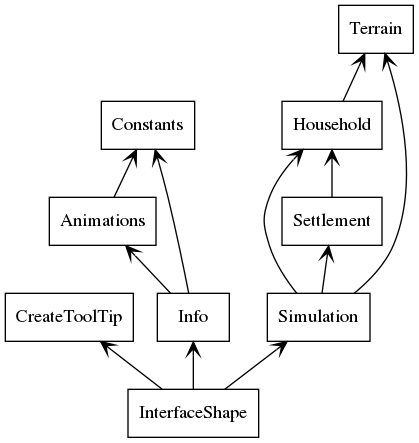
\includegraphics[width=10cm]{packages}
			\caption{Diagram showing the relationship between all the classes involved in the programme.}
			\label{fig:Packages}
		\end{figure}
	
	\section{Test Cases}
		
	\section{Conclusions}
		The application as designed seems to run much faster than its predecessor, while also being written in a more extensible manner. For clients, there are quality of life features that were implemented which were not in the original, for example being able to set up multiple runs of the same settings to automatically continue as well as being able to easily save graphs which are generated. In the original, a single graph could be saved at a time. In the reimplementation, all graphs could be saved at once, or a graph could be zoomed in on before being saved.
	\begin{thebibliography}{9}
		
	\end{thebibliography}

	\appendix
	\section{Manual}
		\subsection{Sliders}
			The left hand side of the interface contains a set of sliders which may be adjusted to give different parameters to the program. On adjustment, the sliders automatically reset the simulation with the changed values. Below sliders are check boxes, which function similarly - resetting the simulation on being changed. One check box asks the users for a seed and then passes this to the simulation.
		
		\subsection{Simulation display}
			The central portion of the interface displays the current state of the simulation, in which the user may right click any block to see a description of the current parameters associated with that block. To clear the display of information when no longer required, the user may left click. The information displayed depends on what type of block was clicked on, as follows:
			\subsubsection{Settlement}
				Settlements are represented by houses, where the size of the house represents the total population of the settlement.\\
				When right clicked on, settlements display their total population, and how many households are contained within.\\
			\subsubsection{Fields}
				Fields are represented by a circle (unharvested) or a piece of barley. The colour of the symbol is related to the colour of the household which has claimed the field, with purple representing the top 33\% of wealth, blue representing the middle 33\% and yellow representing the bottom 33\%.\\
				When right clicked on, fields will display whether or not they have been harvested, their fertility, their potential harvest for the year and the number of years it has been since the field has been harvested.\\
			\subsubsection{Land}
				The shade of green of each of the block of represents its fertility, where a darker colour means that it is more fertile. Right clicking on a piece of land displays its fertility and what its potential harvest would be if it were to be claimed and harvested.
				
		\subsection{Graphs of data}
			Two displays are available on the right hand side of the interface. Each is controlled by a drop down box beneath it which when clicked allows the user to choose one of the eleven graphs to be displayed. There is also a tool bar underneath each graph which allows the user to interact with the graph through actions such as panning or zooming. To save an individual graph one may click the save button in the toolbar. To save all the graphs into a folder of your choosing, click “Save all figures” and enter the name of the folder. 
			
	\section{Technical API Manual}
		This section will assume a familiarity with how the simulation is meant to function as well as the code of Simulation, Settlement, Household and Terrain, although a brief description of their functionality will be described. If additional variables are required in Settlement, Household or Terrain, note that these variables must first be added to the "\_\_slots\_\_" list at the top of the class in order to be used. This is to provide speedup to accessing variables and reduce memory usage overall and is opposed to the usual python dictionary which is used to store variables within classes.
			\subsection{Simulation}
				The Simulation class forms a wrapped for all of the other simulation objects, holding data that is required globally throughout. It also controls some of the order of operations. For extensibility, the simulation class would probably not provide much help outside of changes to instantiation. If one were to want different households or settlements to run with different parameters, this is where one would make the changes.
			\subsection{Settlement}
				The Settlement class holds the households which exist in a specific area together, controls the removal of households when their population reaches 0 and ensures that the households within run their yearly simulations in a random order. If one were to want to change the order in which the simulation is run, or change behaviour of household removal, this is the file in which changes should be made.
			\subsection{Household}
				The Household class controls the year to year activities of individual houses, including farming, using food, population increases and changes to ambition and competency over generations. If one were to want to change any general behaviour of the individual households, this is likely to be the correct area to look. Due to how python treats functions, functions can be replaced in certain households without affecting how all households function. If this is done, it must be ensured that the population of the settlement and total population are adjusted when the population is adjusted, and that the grain of the household at the end of the year is added to the total grain.
			\subsection{Terrain}
				The Terrain class maintains information about the state of the land in a specific position, as well as containing information about what its position is. It is unlikely that extensibility would come from altering this class, but if it is necessary, then it must be ensured that the years not harvested is incremented each year, harvested is set to false at the start of the year, the fertility and harvest are set every year, and the claim and unclaim functions need to maintain their current functionality. 
	\section{Screenshots}
	\begin{figure}[!htb]
		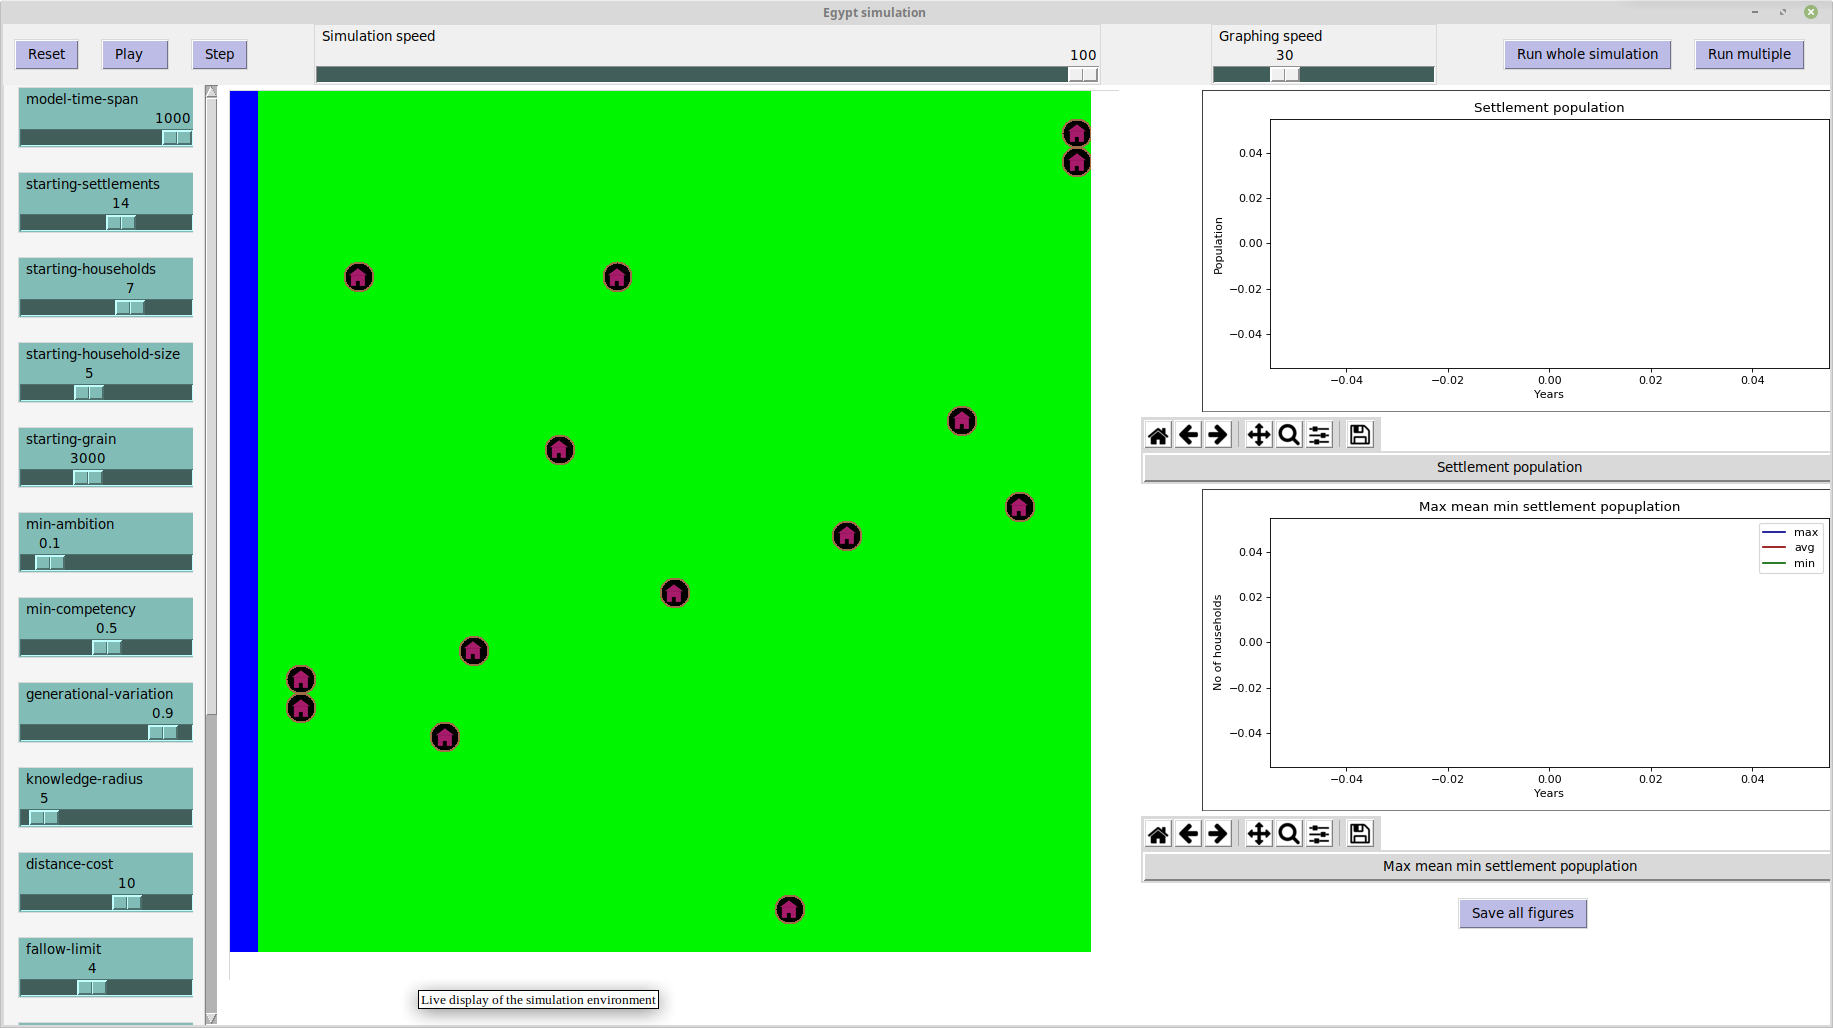
\includegraphics[width=15cm]{OnOpen}
		\caption{Screenshot of the application once opened, without any actions being performed.}
		\label{fig:OnOpen}
	\end{figure}
	
	\begin{figure}[!htb]
		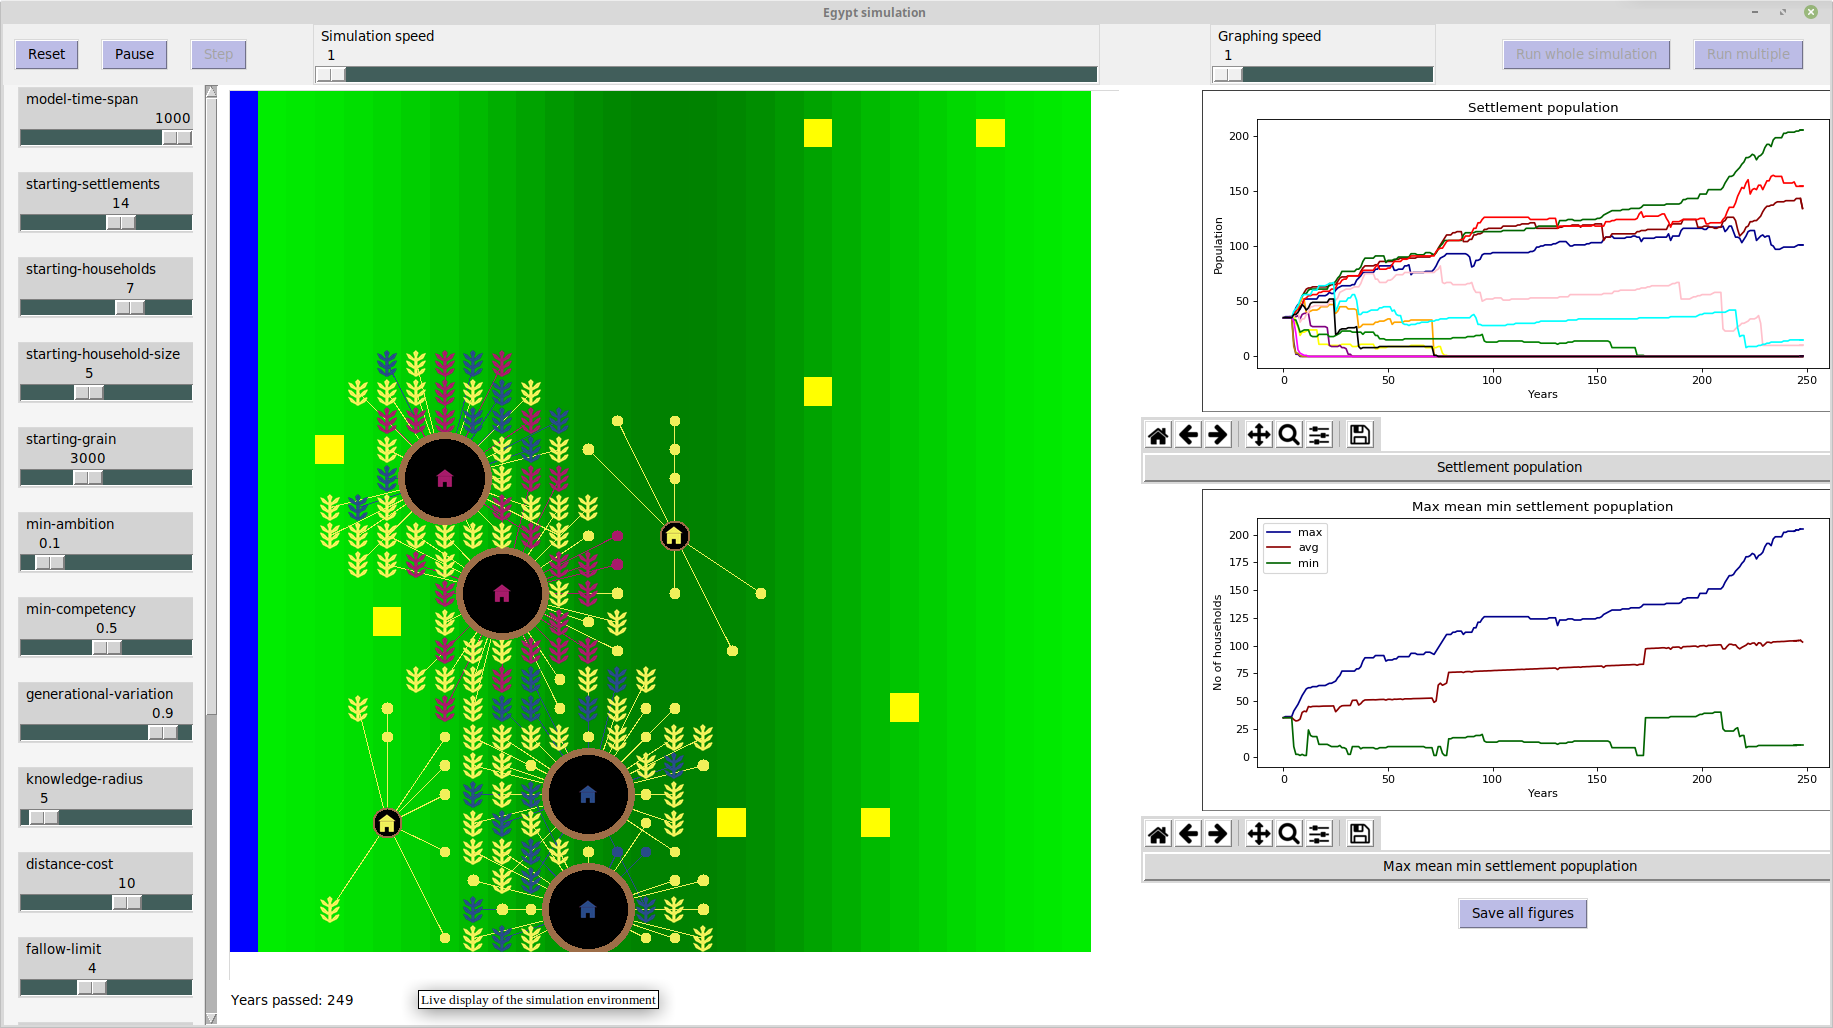
\includegraphics[width=15cm]{WhileRunning}
		\caption{Screenshot of the application once a run has begun, taken at a slow simulation speed to prevent screentearing during a screenshot.}
		\label{fig:WhileRunning}
	\end{figure}
	
	\begin{figure}[!htb]
		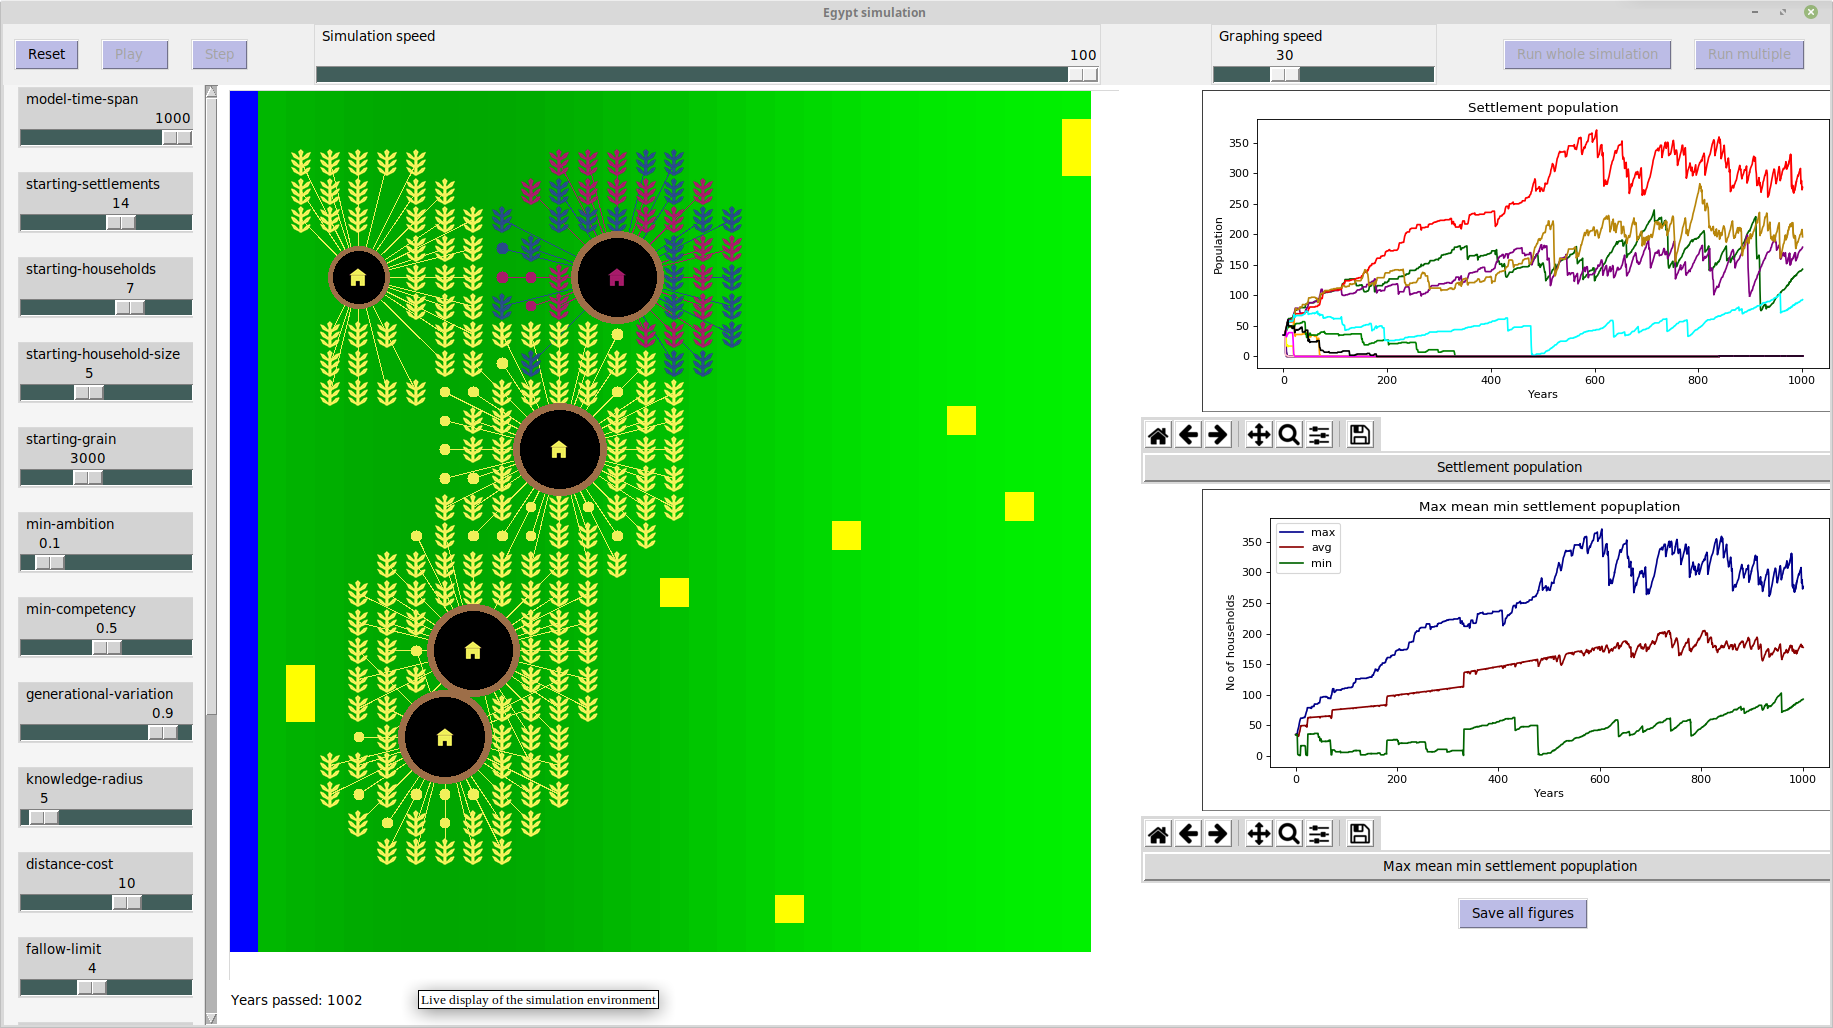
\includegraphics[width=15cm]{FinishedRunning}
		\caption{Screenshot of the application once a run has completed.}
		\label{fig:FinishedRunning}
	\end{figure}
	
	\begin{figure}[!htb]
		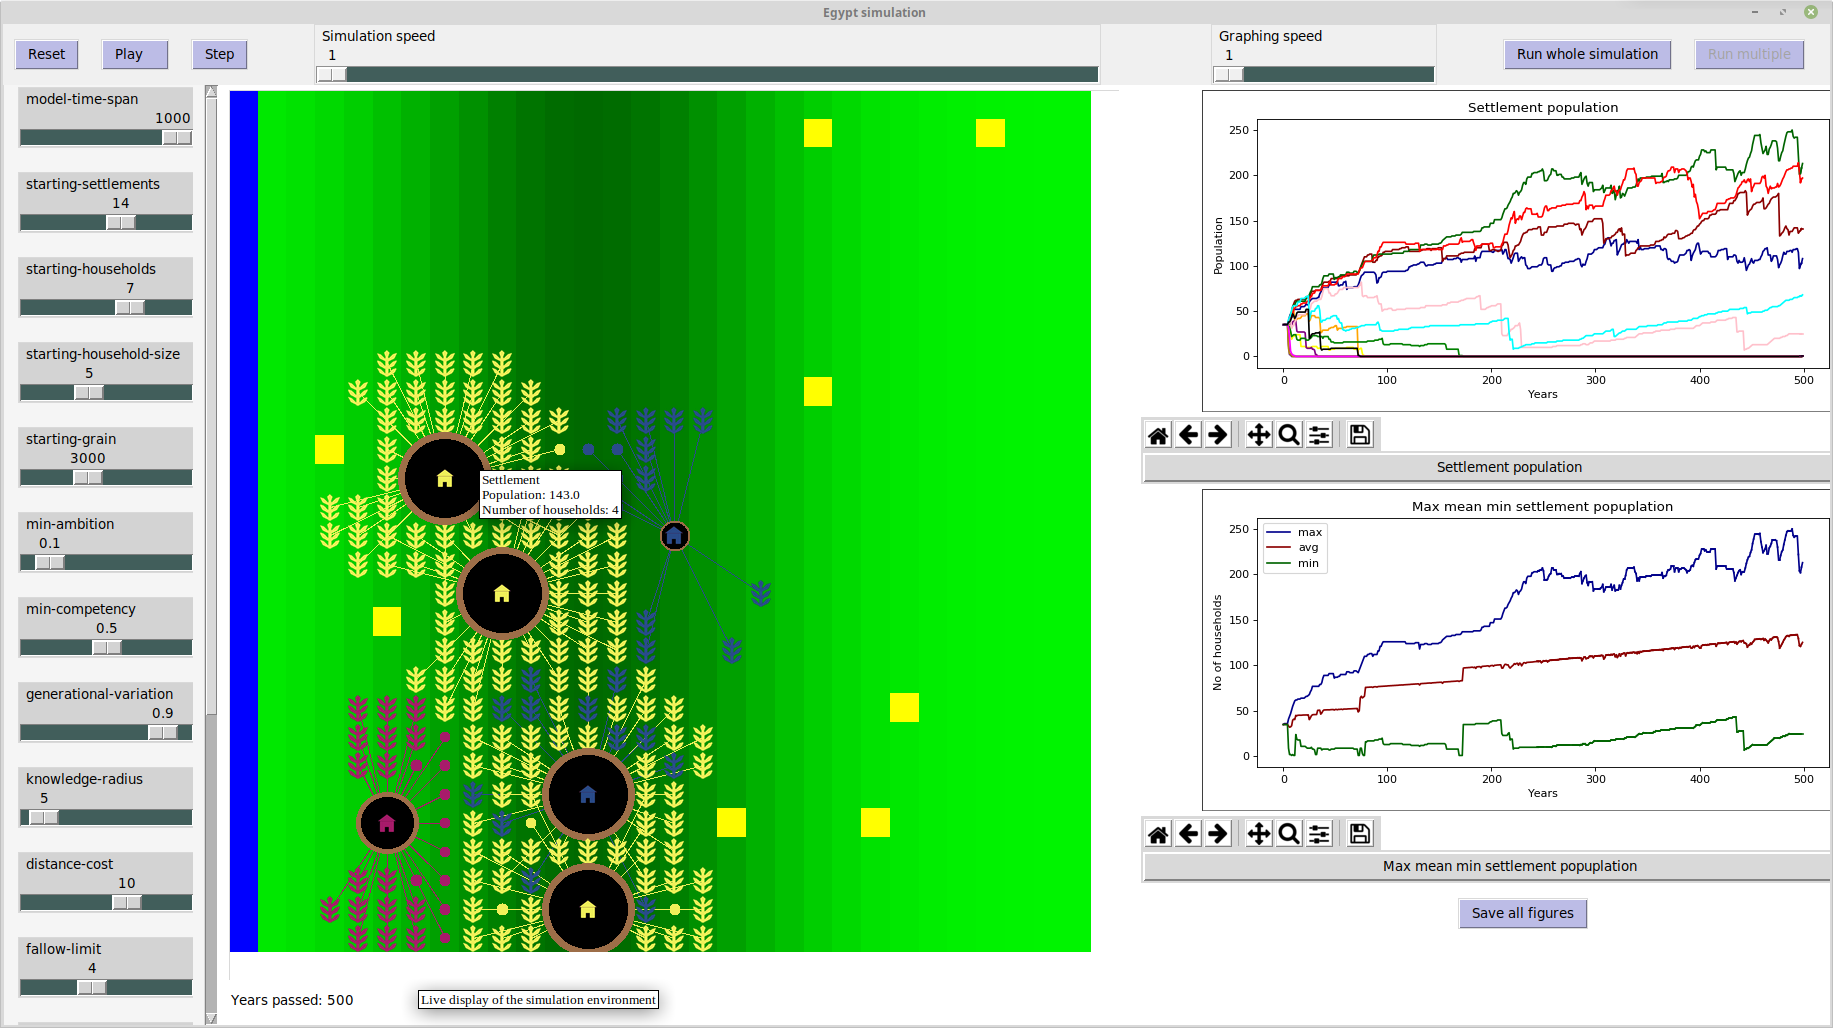
\includegraphics[width=15cm]{RightClickOnSettlement}
		\caption{Screenshot of the application during a run, with the simulation paused and the output of right clicking on a settlement shown.}
		\label{fig:ClickOnSettlement}
	\end{figure}
	
	\begin{figure}[!htb]
		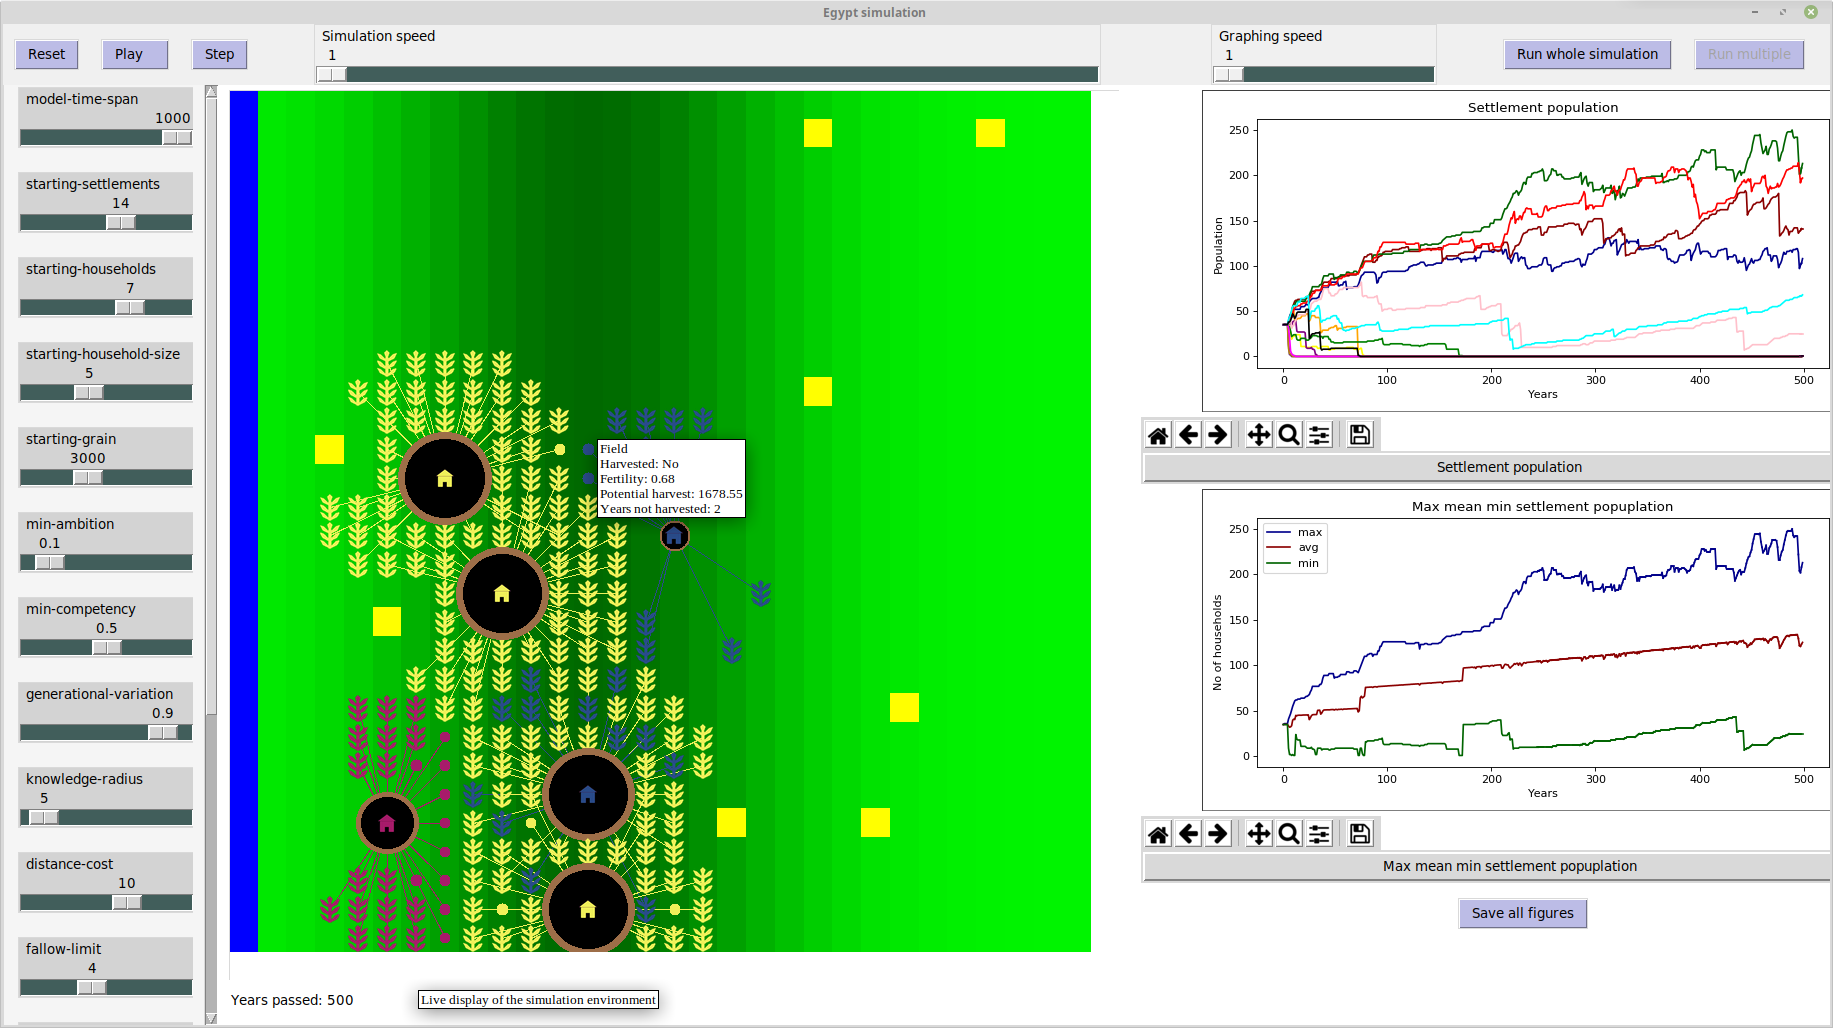
\includegraphics[width=15cm]{RightClickOnNotHarvestedField}
		\caption{Screenshot of the application during a run, with the simulation paused and the output of right clicking on an unharvested field shown.}
		\label{fig:ClickOnUnharvested}
	\end{figure}
	
	\begin{figure}[!htb]
		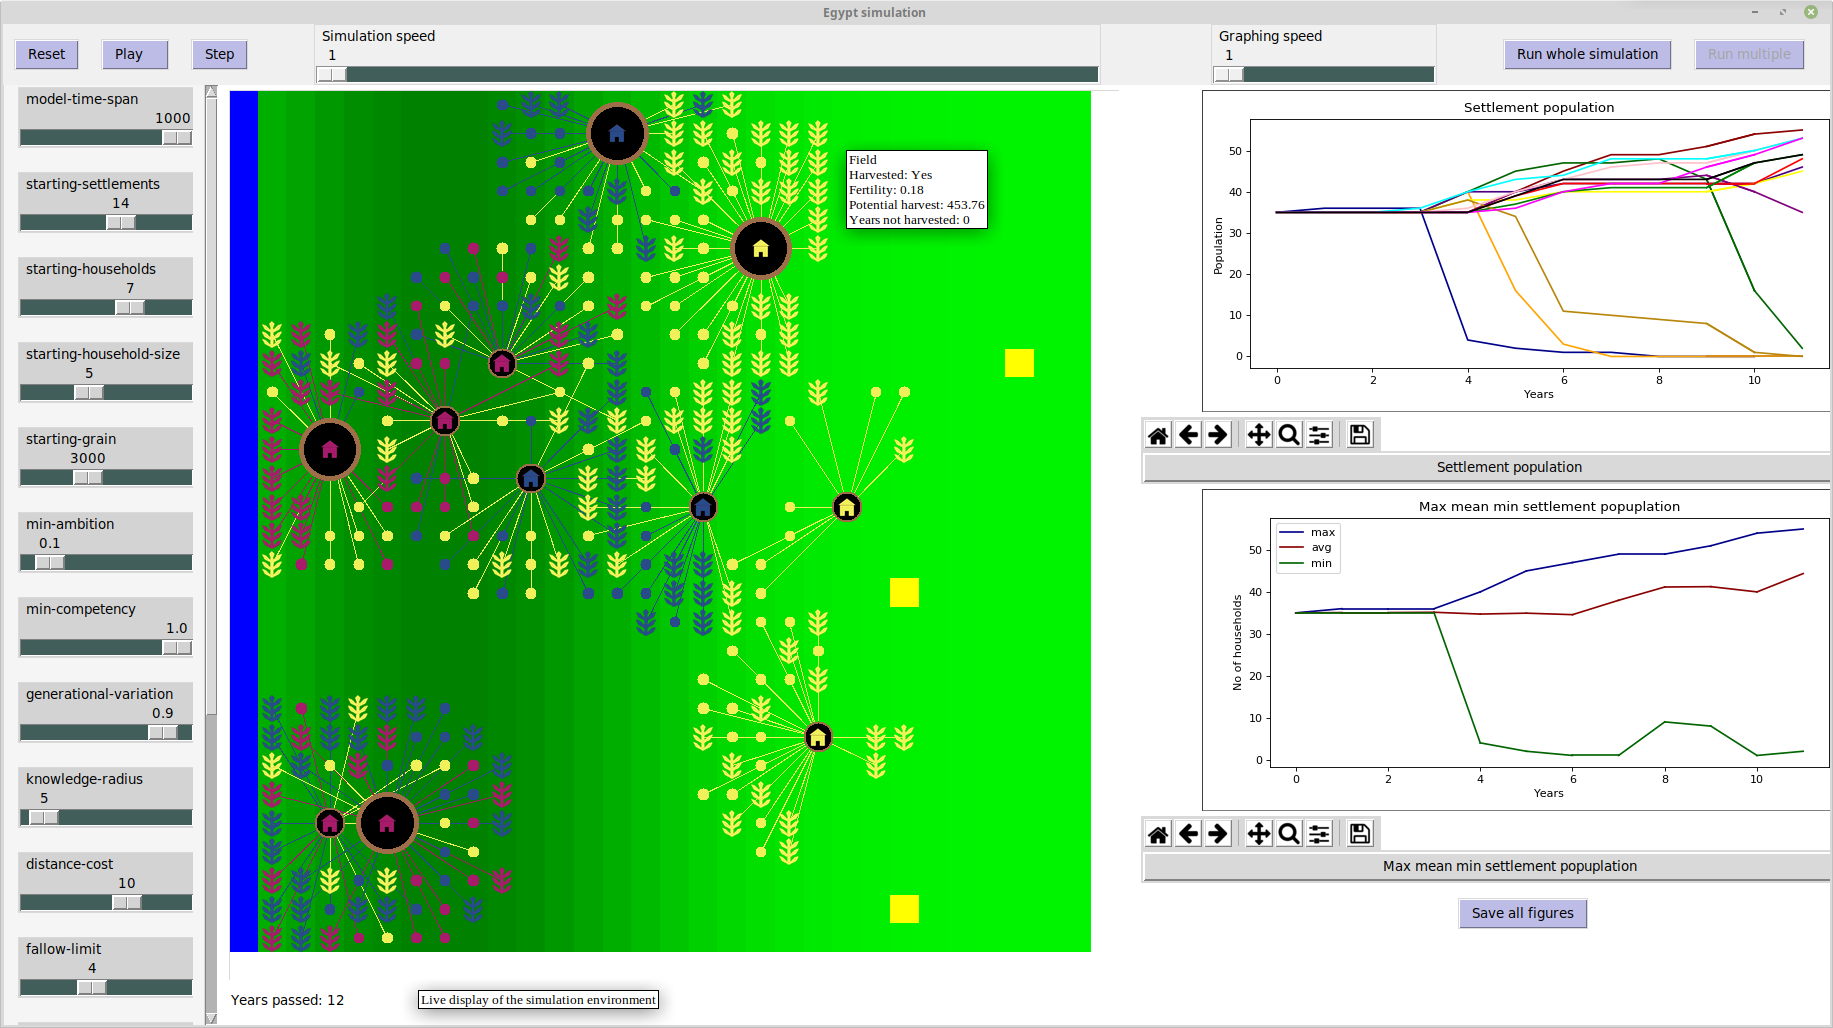
\includegraphics[width=15cm]{RightClickOnHarvestedField}
		\caption{Screenshot of the application during a run, with the simulation paused and the output of right clicking on a harvested field shown.}
		\label{fig:ClickOnHarvested}
	\end{figure}
	
	\begin{figure}[!htb]
		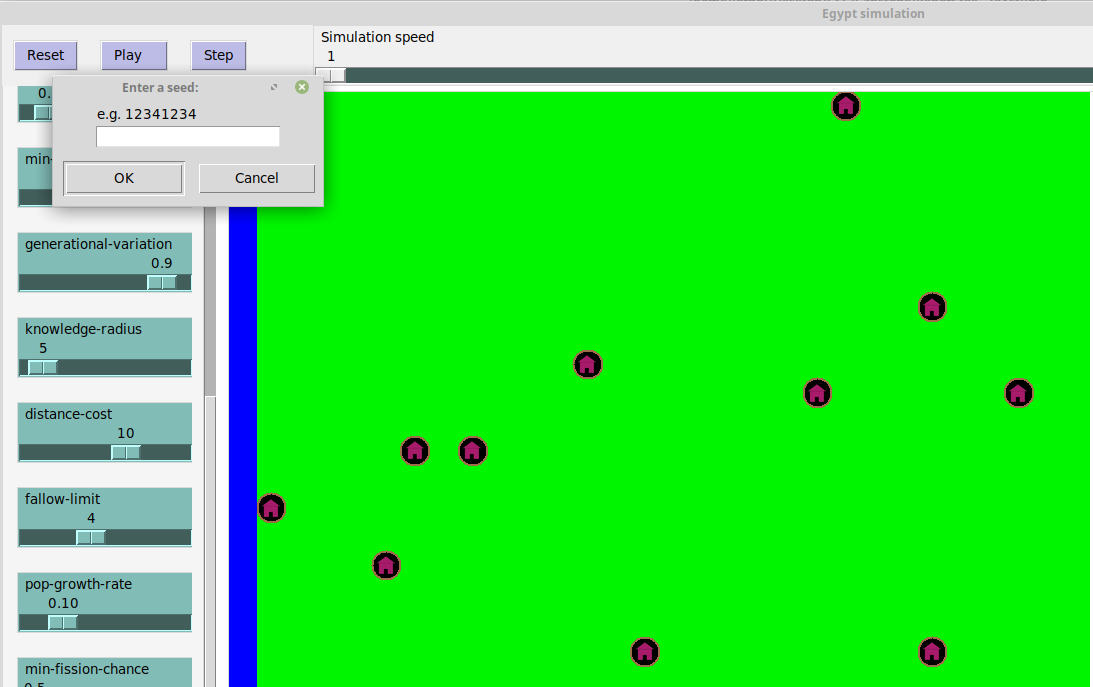
\includegraphics[width=15cm]{SeedEntry}
		\caption{Screenshot of the application showing how a manual seed is entered.}
		\label{fig:Seed Entry}
	\end{figure}
	
	\begin{figure}[!htb]
		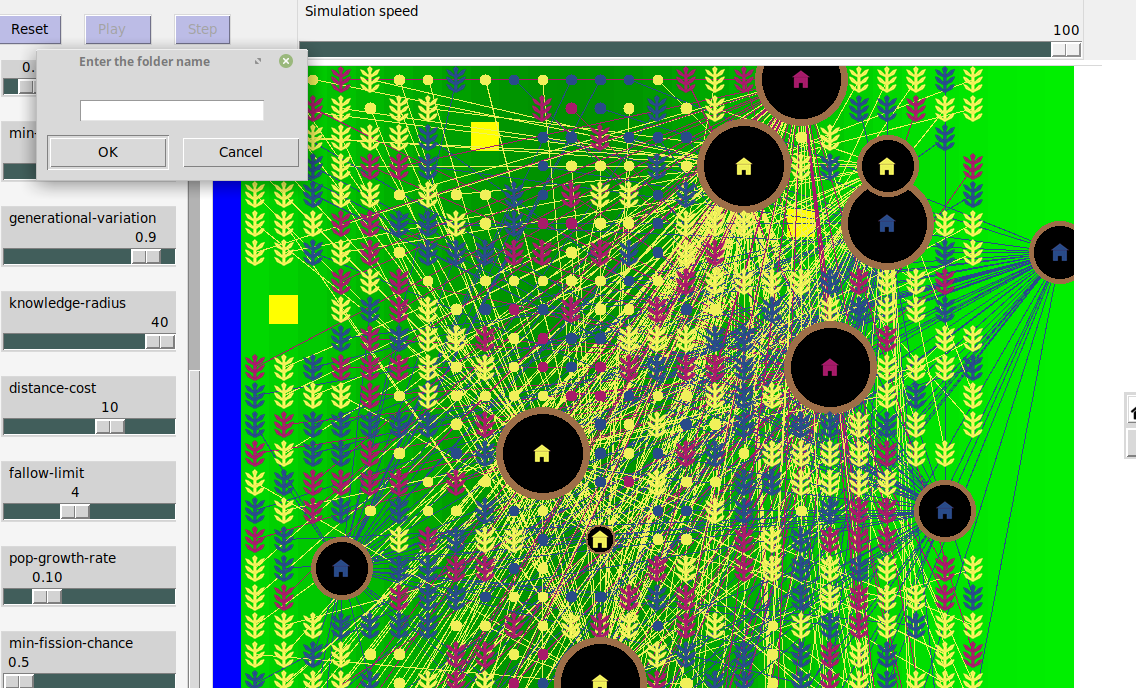
\includegraphics[width=15cm]{SaveAll1}
		\caption{Screenshot of the application showing the dialog asking for a foldername to save multiple figures in for the "Save all Figures" button.}
		\label{fig:SaveAllFolder}
	\end{figure}
	
	\begin{figure}[!htb]
		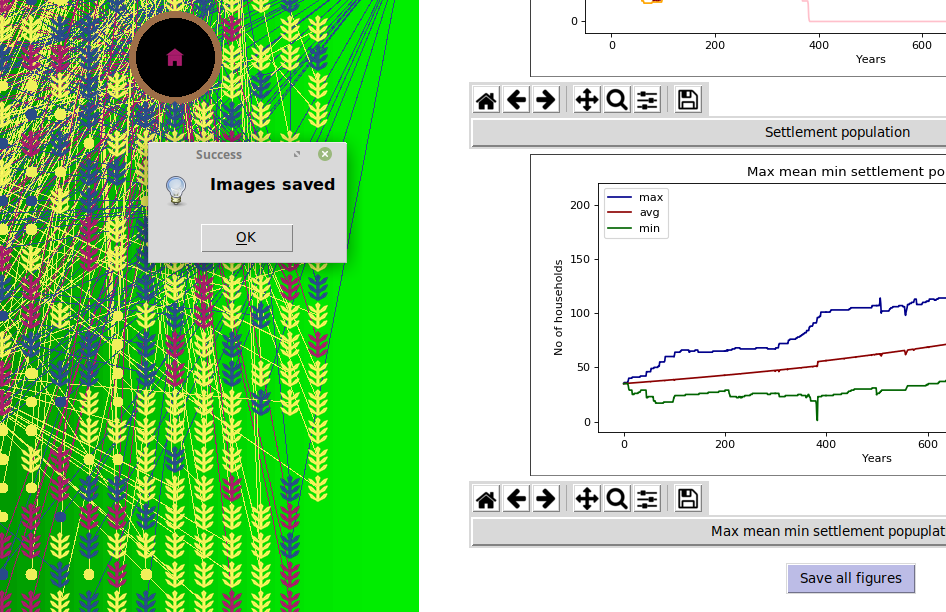
\includegraphics[width=15cm]{SaveAll2}
		\caption{Screenshot of the application showing output of the "Save all Figures" button once all figures have been saved.}
		\label{fig:SaveAllSaved}
	\end{figure}
\end{document}